\chapter{Results and Evaluation}
To evaluate the effect of OS on the overall performance of the network, finding out the correct metrics to measure the performance is very important. The ideal metric are those that correctly reflect the inherent complexity involved in performing the OS Encryption. There are plenty of metrics used to measure the performance of a network. However not all of them are relevant in terms of what we aim to achieve. For example number of packets dropped is a good metric to test out new network protocols, however in our scenario the number of packet drops is not relevant since that attribute is not affected by the implementation of OS Encryption. The MPLS OS switch may drop all the MPLS OS packets if it fails to encrypt or decrypt the packets, however that is a case where the protocol failed as a whole and not a performance issue. Such metrics will be ignored in the evaluation of this project. The metrics that we find are relevant in our scenario are explained in the following sections.
    
\section{Latency}
    Latency is a term used to define the time delay between data communication over a network. Packets flowing through a network take time to reach their destination. The difference between the time a packet is sent from the sender and the time it reaches the receiver is termed as delay. In network communication delay is measured in terms of Round Trip Time (RTT). Due to the difference between the clock time of two nodes in a network it is difficult to measure the exact time a packet take to reach from point A to point B. In network the time it takes for a sender to send a node to a receiver and the receiver to send an acknowledgement back to the user is termed as a round trip time. In this case the user keeps track of the time it sent the data and the time it received an acknowledgement of the data.
    For our experiment we measured the effects of OS on the latency of the network system by comparing it to the one without the OS. The Encryption decryption and addition of special purpose labels is bound to introduce some additional computation time and as such would affect the time required to send and receive the packets. We measured the latency of the system by measuring the Round Trip Time (RTT) of 1000 ICMP ping requests and responses and compare its average, RTT times. It is expected that the RTT for MPLS OS will be more than the traditional MPLS routing. Refer Figure 4.1 for the obtained results.
    \begin{figure}[H]
       \centering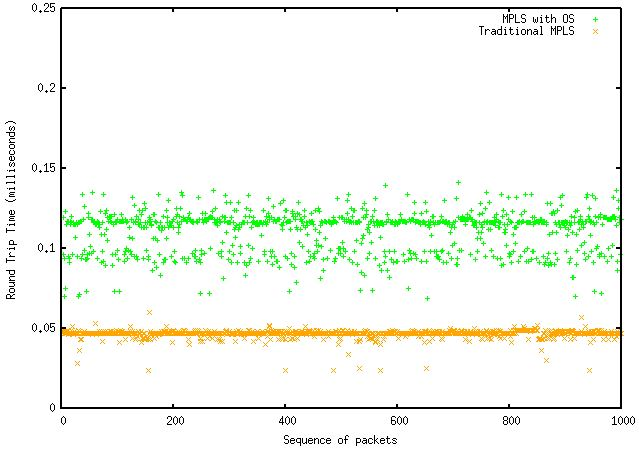
\includegraphics[width=\textwidth]{images/17_MPLSvsOS.JPG}
       \caption{Round Trip Time of Traditional MPLS and MPLS with OS}
       \label{fig:compbest}
\end{figure}
    As stated in Figure 4.1 we can see that the average RTT for MPLS OS is infact slightly more than the average RTT of the traditional MPLS network. IT was also observer that a small number of packets cluster together at a RTT slightly less that 0.1 millisecond and deviate from the majority of the MPLS with OS packets in the graph. It is difficult to find out why a small number of packets face the same lower RTT than majority of the packet. Further study may be needed to find out. A difference of about 0.07 milliseconds was observed between the RTT of MPLS with OS packets against traditional MPLS packets. Though the difference is not that significant we can confirm that the Encryption and Decryption process does in fact add more computational time to the overall time required for data transfer.
    
\section{Effects of Size of Packets}
Based from our results in the previous section we can assume that the amount of RTT taken by a packet may be proportional to the amount of data that needs to be encrypted and decrypted. More the data more time required to encrypt and decrypt it. It would be interesting to measure how the increase in packet size might affect the time taken to encrypt and decrypt and thus affect the RTT.


\begin{figure}[H]
       \centering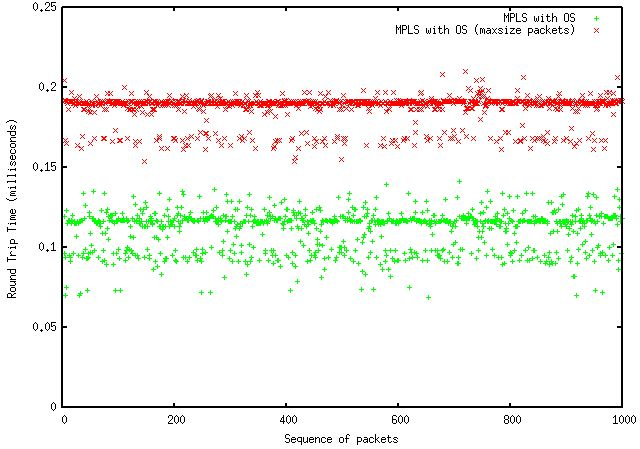
\includegraphics[width=\textwidth]{images/19_MAXOSvsOS.JPG}
       \caption{Round Trip Time of MPLS OS with 56 byte ping packet vs MPLS with OS with Maximum Packet Size 1500 bytes}
       \label{fig:compbest}
\end{figure}

    In Figure 4.2 we see that the latency of MPLS OS increases by an additional 0.7 milliseconds approx if the packet size was increased to to the Maximum Transfer Unit MTU as compared to a ping packet of default size of 56 bytes plus 20 bytes of MPLS OS headers (MEL, CW, additional Cipher text).
    If we compare the MPLS OS results with traditional MPLS packet with the packet size reaching the MTU we can see that the MPLS with max packet size still has lesser latency than MPLS with OS with a default 56 byte size packets. Refer figure 4.3 for the details.
    
   \begin{figure}[H]
       \centering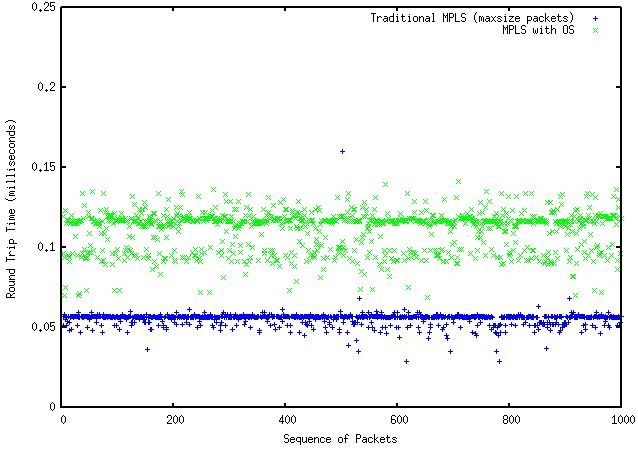
\includegraphics[width=\textwidth]{images/24_MaxMPLSvsOS.JPG}
       \caption{Round Trip Time of Traditional MPLS with max size packets vs MPLS with OS with regular size packets}
       \label{fig:compbest}
\end{figure}

Figure 4.4 summarises the average latency in all the 4 systems.

\begin{figure}[H]
       \centering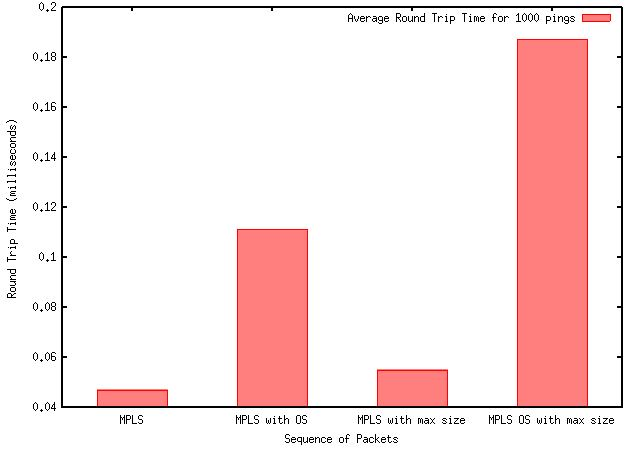
\includegraphics[width=\textwidth]{images/21_Average.JPG}
       \caption{Average Latency in all the four Systems}
       \label{fig:compbest}
\end{figure}
    
\section{Packet Size Limitation}
The Maximum Transmission Unit (MTU) is the size of the largest packet that can be communicated into a network. Packets whose size exceeds the MTU undergo IP fragmentation where the packet is broken down into small chunks that can be transmitted into the network. The default MTU for Ethernet is set to 1500 bytes of data, exceeding which if the packets are IP packets, IP fragmentation takes place.
	MPLS do not undergo IP fragmentation if the packet size increases beyond the 1500 bytes allowed on the Ethernet. As we observed, MPLS adds an additional of 4 bytes of data per label pushed on the data packet. Thus care needs to be taken not to max out the packet size if it expected to flow down an MPLS network.
    This concern is more intensified in an MPLS OS network. OS adds an additional overhead data to the data packet comprising of the CW, the MEL and the special purpose MPLS label as well as the 16 bytes larger Cipher text data. This means that the data packet that is going to flow through an MPLS network implementing OS has to compensate for the additional data overheads by making sure the application data payload is small in size so as to not exceed the MTU.
    This also states that the amount of data that can be transferred over an MPLS OS network in a given time frame will always be less than data transferred in traditional MPLS network. This case can be best tested using throughput/bandwidth measuring tools like 'iperf'. We tried performing this test on the OS system, however it was observed that 'iperf' would crash the system when it was run, freezing the virtual box in which the test was being performed. Further analysis and debugging will be needed to figure out the issue.

